\chapter{Theory}
\label{chapter:theory}

% • Does the candidate show sufficient familiarity with, and understanding and criti-
% cal appraisal of, the relevant literature?
% • Does the thesis provide a sufficiently comprehensive investigation of the topic?

\section{The atmosphere under greenhouse gas forcing}
climate sensitivity
\parencite{jeevanjeeClimateSensitivityRadiativeconvective2023}
radiative equilibrium
forcing and feedback
tropospheric warming
Why is the troposphere warming under greenhouse gas forcing?
What is the warming structure? How can we explain it?
Enhanced upper tropospheric warming in the tropics
Arctic amplification

stratospheric cooling
Why is the stratosphere cooling under greenhouse gas forcing?

\section{Hadley circulation strength under greenhouse gas forcing}
\subsection{Definition of the Hadley cell}
The HC can be evaluated by its strength and extent, which can be determined by calculating the mass stream function (MSF)
\begin{equation}\label{eq:msf}
    \psi_\mathrm{max}=\frac{2\pi a\cos\varphi}{g}\int^0_{p_\mathrm{s}}\bar{v}\mathrm{d}p'.
\end{equation}
The MSF is always parallel to the flow in the vertical $p$--$\varphi$ plane. A positive value of $\psi_\mathrm{max}$ indicates a clockwise circulation and a negative value a counter-clockwise circulation. In the annual mean, the Northern hemisphere shows a clockwise and the Southern hemisphere counter-clockwise circulation. Since the Hadley cell vertically integrates the mass flux, its values symbolize the net magnitude of mass transport above and below and to the right and the left of a certain grid point. At the HC maximum the integral covers exactly the upper or lower branch of the circulation. In the literature, one can find several different metrics for the HC strength. Some use the MSF at a fixed pressure level or spatially average, while others use the minimum of the vertical pressure tendencies $\omega$. HC trends have show a large sensitivity to the metric used \parencite{pikovnikMetricsHadleyCirculation2022}. We find it most plausible to calculate the strength of the HC from the maximum of the $\psi_\mathrm{max}$ and the extent from the latitude at which $\psi_\mathrm{max}$ becomes zero, averaged between $300$ and $\SI{700}{hPa}$. Thus, all our calculations use this metrics while referenced studies may use a different one.
The global HC, as depicted in Figure \ref{}, cannot be found at any given longitude but rather you have a lot of different regional HCs, which are strongly influenced by the shape and the distribution of continental land mass. HC trends might be different depending on the region of the HC that is considered. This study will only consider the global HC and, if not stated differently, its annual mean.
\subsection{Historical and projected Hadley cell trends}
The HC has been changing already since the beginning of the satellite era.
Observational datasets using outgoing longwave radiation, precipitation, and sea level pressure as proxies for the HC position have shown a significant widening of the HC in the historical period (1979-2000s) \parencite{huObservationalEvidencePoleward2011}. Depending on the observed quantity the widening has a magnitude of \SIrange{1.2}{4.0}{\degree}. Similar trends have also been found in reanalysis data \parencite{huObservedPolewardExpansion2007}. 
In phase 6 of the Coupled Model Intercomparison Project (CMIP6) "All-forcing" experiments also found that the Hadley cell widened in the period 1970-2014 of $\SI{0.65}{\degree} \pm \SI{0.02}{\degree}$ per decade. This is much smaller than the trends obtained from observational records. The influence of natural variability is highlighted in this context. The widening in CMIP6 models is found to be larger in the Southern hemisphere. The primary driver of the historical widening is greenhouse gases forcing. Changes in anthropogenic aerosol forcing and stratospheric ozone only contribute to Southern hemisphere HC changes \parencite{xiaComparisonTrendsHadley2020}.

In terms of the HC strength, studies found opposing trends in climate models and reanalysis data in the historical period for the Northern hemisphere. While CMIP5 models show a robust weakening of the NH HC, the reanalysis data even suggests a strengthened. This discrepancy is not due to internal variability but rather stems from a misrepresentation of latent heating in the reanalysis \parencite{chemkeOppositeTropicalCirculation2019}. According to CMIP6 models, greenhouse gas forcing leads to a weakening in both hemispheres, with stratospheric ozone, and aerosol forcing contributing to a net modest strengthening in the southern hemisphere. This strengthening trend had not been observed in the previous CMIP5 models. The annual mean Northern hemisphere HC weakened by approximately $5\%$ in over 1970-2014  \parencite{xiaComparisonTrendsHadley2020}. 

CMIP6 projections of the HC extent show that the widening trend of the HC increase with radiative forcing in both hemispheres. This increase is stronger in the annual mean Southern hemisphere HC while showing no seasonality. The strength of the SH HC is not projected to change with radiative forcing. In the NH, there is a projected net weakening of the annual-mean maximum of about $10\%$ over the period of 2016-2100 \parencite{xiaComparisonTrendsHadley2020}. Consistent with the historical simulation the largest contributor to the change is expected to be the increase in future \CO{} concentrations in the atmosphere. 

\subsection{Drivers of HC changes}
Several mechanisms have been proposed to explain HC weakening. There are two mechanisms relating the weakening of the HC to the direct effect of \CO{} increase in the atmosphere. Direct means only considering \CO{} effect on radiative transfer without its influence surface temperature changes with their corresponding feedbacks. Around 81\% of the net radiative cooling of the atmosphere is balanced by latent heating which poses a constrain on the precipitation rate \parencite[p. 35]{GlobalPhysicalClimatology2016}. \textcite{bonyRobustDirectEffect2013} argue that by increasing the \CO{} in the atmosphere, the loss of infrared radiation to space is reduced. This warms and stabilizes the atmosphere weakening upward motions, i.e., the circulation. The second mechanism employs the the spatial structure of \CO{} forcing. In regions of ascending motion, such as the equator, the \CO{}  radiative forcing is reduced. This is due to the presence of deep-convective clouds and the high humidity, which both are effective longwave absorbers. Thus, \CO{} below cloud top or the moist atmosphere has a limited effect on OLR (I think this argument is wrong because \CO{} band vs. water vapor absorption region). In subsiding regions, such as the subtropics, the \CO{} radiative forcing is larger because this effect is missing. Given a larger forcing in the extra-tropics than at the equator, less energy transport and also a weaker circulation is required. About 15\% of the century scale weakening is attributed to the direct effect of \CO{} using fixed-SST simulations \parencite{merlisDirectWeakeningTropical2015}.

Another mechanism compares the change in saturation vapor pressure according to the Clausius-Clapeyron (CC) equation to the changes in precipitation. Assuming that the global mean precipitation is given as 
\begin{equation}
    P = Mq
\end{equation}
where $M$ is the convective mass flux and $q$ is a typical boundary layer mixing ratio, which scales with the CC equation. In its linearized form, one obtains the following expression for the change in mass flux
\begin{equation}
    \frac{\delta M}{M} = \frac{\delta P}{P} -\frac{\delta q}{q}.
\end{equation}
Inserting typical global mean values for ${\delta P}/{P}=0.03\delta T$ (where does this value come from? simulations?) and with CC ${\delta q}/{q}=0.07\delta T$ gives a mass flux change of ${\delta M}/{M}=-0.04\delta T$, a weakening of global circulations
\parencite{heldRobustResponsesHydrological2006}. This relationship holds better for global zonal circulations, e.g., the Walker circulation, than the HC \parencite{vecchiGlobalWarmingWeakening2007}.
\textcite{seoMechanismFutureChanges2014} used the axisymmmetric scaling (see next section) to predict the HC strength changes via changes in the meridional temperature gradient, static stability, and tropopause height. They found the meridional temperature gradient to have the largest correlation.
Using the quasi-geostrophic Kuo-Eliasson equation allows us to isolate effects that contribute to HC changes \parencite{vallisResponseLargescaleStructure2015}. According to this equation diabatic heating, eddy heat flux, eddy momentum flux, zonal friction and static stability changes capture the response of the change in maximum MSF. None of these factors alone can fully explain the changes but the most important contribution comes from an increase in static stability with diabatic heating changes even contributing to a strengthening of the HC on longer time scales \parencite{chemkeElucidatingMechanismsResponsible2021}.
For a comprehensive evaluation and comparison of the different proposed HC weakening mechanisms, one should consult
\parencite{chemkeElucidatingMechanismsResponsible2021}.

Investigating the influence of different feedback mechanisms in shaping the HC response to climate change 
\parencite{feldlCharacterizingHadleyCirculation2016}
Correlation study \parencite{dagostinoFactorsControllingHadley2017}
\section{The angular momentum budget}
Considering the angular momentum budget of the Earth, one addresses the fundamental question of why there is a meridional circulation in the atmosphere in the first place. An answer is provided by the axisymmetric theory of \textcite{heldNonlinearAxiallySymmetric1980}. It also provides a scaling for the HC strength and extent linking it directly to thermodynamical parameters. Because this theory ignores eddies, we are further investigating their effect on the HC in the following subsection. Since there is no unifying theory incorporating angular momentum conservation and angular momentum transport by baroclinic eddies, we introduce the energetic budget framework of the HC to explain why it changes. This is a more diagnostic framework which does not explain the existence of the HC from first-hand principles but rather takes the necessity transport energy poleward as granted. This necessity can be inferred from observational data of the TOA radiative imbalance showing an excess of incoming radiative fluxes relative to the outgoing radiation at the equator and vice versa at higher latitudes. This transport by the the atmosphere can be split up into a mean component, i.e., the HC in the tropics, and and eddy component.

\subsection{Drivers of Hadley cell widening}

\subsection{Axisymmetric theory}\label{sec:axisymmetric}
The axisymmetric theory considers a flow in the $\varphi$--$z$ plane with no meridional circulation ($v=w=0$). This prevents the existence of large scale barotropic or baroclinic eddies. The questions why there is a meridional circulation in the first place is answered by the axisymmetric theory \parencite{heldNonlinearAxiallySymmetric1980}. This question is raised because one could imagine a world where Earth is just in radiative equilibrium everywhere. This means that every point on Earth emits just as much radiation as it receives from the sun. Thus, there would not be any meridional temperature or energy transport necessary.
Given a radiative-equilibrium temperature profile of the Earth
\begin{equation}
    \frac{\theta_E}{\theta_0}=1-\frac{1}{3}\Delta_h(3\sin^2\varphi-1)+\Delta_v\left(\frac{z}{H}-\frac{1}{2}\right)
\end{equation}
(see Figure \ref{fig:held_hou_T}), one can obtain a corresponding zonal wind $u_E$ via the thermal wind relationship. Here, $\Delta_h$ is the fractional pole to equator temperature difference, $\Delta_v$ the fractional temperature difference between the surface and the top of the fluid, $H$ the depth of the fluid, and $\theta_0$ the global mean value of $\theta_E$. This solution not only produces westerly winds at the equator, which are not observed in the atmosphere, but also violate Hide's theorem \parencite{hideDynamicsAtmospheresMajor1969}. Hide's theorem states that a maximum of angular momentum within the flow domain cannot be sustained due to dissipation within the flow. A maximum of angular momentum can only exist at the boundaries. This tells us that this RE temperature profile is not able to persist on Earth and that we require some poleward transport of energy.

The conservation of angular momentum
\begin{equation}
    M=(u+\Omega a\cos\varphi)a\cos\varphi
\end{equation}
provides a second constraint for a HC solution with the zonal wind $u$, $a$ being the radius and $\Omega$ the rotational frequency of the Earth. The angular momentum conserving wind can then be derived as
\begin{equation}
    u_M=\Omega a\frac{\sin^2\varphi}{\cos\varphi}.
\end{equation}
This allows us to infer, via the thermal wind relationship, a temperature profile $\theta_M$ (see Figure \ref{fig:held_hou_T}), which is now slaved to angular momentum conservation. Assuming that the energy is conserved in the upper branch and that the solution is continuous at the edge of the HC, allows us to determine the undefined parameters of this solution. One also obtains a finite scaling for the HC width
\begin{align}
    \phi_H&\sim\left(\frac{gH\Delta_h}{\Omega^2a^2}\right)^{1/2}
\end{align}
and for its strength
\begin{align}
    \psi_\mathrm{max} &\sim \frac{1}{\tau}\frac{g^{3/2}(H\Delta_h)^{5/2}}{\Delta_v a^2\Omega^3}
\end{align}
where $g$ is the gravitational acceleration of Earth and $\tau$ is the time scale at which $\theta$ relaxes to $\theta_E$.

\begin{figure}[H]
     \centering
     \begin{subfigure}[b]{0.45\textwidth}
         \centering
   
\includegraphics[width=1.0\textwidth,keepaspectratio,trim=0 0 0 0, clip]{literature/temperature_vallis.png}
    \caption{ Radiative-equilibrium temperature $\theta_E$ and angular-momentum-conserving temperature $\theta_M$.}
    \label{fig:held_hou_T}
     \end{subfigure}
     \hfill
     \begin{subfigure}[b]{0.45\textwidth}
         \centering
   
\includegraphics[width=1.0\textwidth,keepaspectratio,trim=0 0 0 0, clip]{literature/zon_vel.png}
    \caption{ Radiative-equilibrium zonal wind $u_E$ and angular-momentum-conserving zonal wind $u_M$. }
    \label{fig:held_hou_u}
     \end{subfigure}
        \caption{Latitudinal profiles of temperature and zonal wind under radiative equilibrium and under angular momentum conservation, adapted from \textcite{vallisAtmosphericOceanicFluid2017}.}
        \label{fig:three graphs}
\end{figure}
% \begin{figure}[H]
%     %% trim=left bottom right top,
%     \centering
%    
\includegraphics[width=0.5\textwidth,keepaspectratio,trim=0 0 0 0, clip]{literature/temperature_vallis.png}
%     \caption{ \parencite{vallisAtmosphericOceanicFluid2017} }
%     \label{fig:held_hou_T}
% \end{figure}
The key contribution of this theory is to explain why there is a HC with finite width in the first place. It also shows that the HC does not extent from the equator to the poles. Subsequent studies have advanced this theory also to temperature profiles which have their maximum off the equator, in order to account for seasonal variations \parencite{lindzenHadleyCirculationsZonally1988}. In our axisymmetric model, the HC is weaker in equinox conditions than observed, leading to the suggestion that the HC in the annual mean is not close to equinox conditions but rather that the HC flips between solstitial states. More recent studies have addressed this discrepancy using eddy permitting models \parencite{walkerResponseIdealizedHadley2005}. In these models, the strength of an annually averaged Hadley circulation is comparable to the Hadley circulation driven by an annually averaged heating. This means that the HC in its equinox state resembles very much an annual mean HC. This highlights the importance of eddies in driving the HC strength, which will be covered in the next section.  


\subsection{Eddy driven mean circulation}
The importance of eddies in shaping the HC was acknowledged even before the axisymmetric theory was developed \parencite{kuoFORCEDFREEMERIDIONAL1956}. More recent studies have compared axisymmetric models to eddy permitting simulations to determine the importance of eddies in altering HC strength \parencite{walkerEddyInfluencesHadley2006,singhEddyInfluencesStrength2017}. They have found that the eddies increase the HC strength by 50--75\%, depending on the model.

From the eddy perspective the HC edge is set by the latitude at which the zonal winds become baroclinically unstable. Baroclinic instability arises due to large vertical shear in a flow. Using a two layer model, one can derive the HC edge as \parencite{Held2000}

\begin{equation}
    \phi_H\sim\left(\frac{NH_e}{\Omega a}\right)^{1/2}
\end{equation}
with $N$ being the Brunt-Väisälä frequency and $H_e$ the depth of the troposphere in the extratropical regions. Correlating the HC edge with tropical tropopause height and extratropical tropopause height in CMIP models has shown that the HC edge is set by the extratropical tropopause height \parencite{luExpansionHadleyCell2007} instead of the tropical tropopause height. This favors an eddy driven perspective of the HC edge.

To quantify HC strength changes from the eddy perspective, we apply a Reynolds decomposition on the zonal and meridional wind. We obtain the eddies as deviations in time from the zonal and temporal mean flow
\begin{equation}
    u=\bar{u}+u',\quad v=\bar{v}+v'.
\end{equation}
These deviations are associated with weather and Rossby waves in the mid-latitudes.
Inserting this into the zonal momentum equation and neglecting viscous forces and vertical advection, we obtain 
\begin{equation}
    \label{eq:eddy_divergence}
    f\bar{v}(1-Ro)=\frac{1}{a\cos^2\varphi}\frac{\partial (\cos^2\varphi\ \overline{u'v'})}{\partial\varphi} + \frac{\partial\overline{u'\omega'}}{\partial p}. 
\end{equation}
Here, the Rossby number is 
\begin{align}
    Ro=\frac{\bar{\xi}}{f}
\end{align}
where $\xi=\hat{k}\cdot\nabla\times\vec{u}$ is the relative vorticity.
Equation \eqref{eq:eddy_divergence} has two limits. For $Ro\to 1$, the left-hand side becomes zero and the eddy term becomes negligible. This means that our Hadley circulation is driven by directly by thermal driving and is close to angular momentum conservation
\begin{align}
    \frac{\partial \overline{M}}{\partial \varphi} = 0
\end{align}
as described by the axisymmetric solution in Section \ref{sec:axisymmetric}. For $Ro\to 0$, the meridional wind $\bar{v}$ is instead balanced by the eddy momentum flux convergence. This regime can be understood as eddy-driven (see Figure \ref{fig:eddy_driven_HC}). For the intermediate $Ro$, there does not yet exist a dynamical theory \parencite{schneiderGeneralCirculationAtmosphere2006}.

\begin{wrapfigure}{r}{7cm}
    %% trim=left bottom right top,
    \centering
   \includegraphics[width=7cm,keepaspectratio,trim=0 0 0 0, clip]{literature/eddies_HC_vallis.png}
    \caption{\parencite{vallisAtmosphericOceanicFluid2017}  }
    \label{fig:eddy_driven_HC}
\end{wrapfigure}
The climatological divergence of eddy momentum flux, which is observed in the tropics, requires a positive mean meridional wind. This holdseven if the zones of baroclinic instability lie well poleward of the HC edge because Rossby waves can propagate into the HC, producing a poleward momentum flux. At the HC edge there is $\bar{v}=0$ and thus no eddy momentum flux. The eddy momentum flux divergence also explains the equatorward meridional wind in the eddy-driven Ferrel cell in mid-latitudes. Over the seasonal cycle, the Rossby number varies between 0.2 and 0.8, approaching either of the two limits. During the equinoxes the Rossby number is small which indicates a strong eddy influence. During the solstices the Rossby number is closer to $1$ in the winter HC but still small in the summer HC.

Assuming that the HC is entirely eddy driven ($Ro=0$), the HC strength can be predicted from the eddy momentum flux by inserting Equation \eqref{eq:eddy_divergence} into the Equation \eqref{eq:msf}. Following \textcite{walkerEddyInfluencesHadley2006}, this gives the integrated eddy momentum flux divergence
\begin{equation}
    \psi_\mathrm{max}=\frac{2\pi a\cos\varphi}{fg}\int^0_{p_\mathrm{max}}\left(\frac{1}{a\cos^2\varphi}\frac{\partial (\cos^2\varphi\ \overline{u'v'})}{\partial\varphi} + \frac{\partial\overline{u'\omega'}}{\partial p}\right)\mathrm{d}p'\equiv \mathcal{T} 
\end{equation}
with $p_\mathrm{max}$ being the pressure level at which the MSF becomes maximum and the Coriolis parameter $f$. The quantity $\mathcal{T}$ is a predictor for the HC strength given a certain eddy momentum flux divergence. This predictor has been shown to be skillful in predicting the HC strength in eddy permitting models for various climates \parencite{walkerEddyInfluencesHadley2006}. 

DRY!!!


\section{The energy budget of the atmosphere}
The energy budget analysis provides diagnostic perspective on the HC. It cannot explain why the Earth is not in radiative (convective) equilibrium but assumes the necessity for poleward transport as given. Using TOA radiative fluxes (see Figure \ref{fig:irradiance}), one can infer that the short-wave radiative flux at the equator is much larger than the emitted outgoing long wave radiation. The opposite is true for the poles. This implies an poleward energy transport by the atmosphere and the ocean. 
\begin{figure}[H]
    %% trim=left bottom right top,
    \centering
   
\includegraphics[width=0.8\textwidth,keepaspectratio,trim=0 0 0 0, clip]{initial_plots/irradiance.png}
    \caption{ }
    \label{fig:irradiance}
\end{figure}
For every column of the earth system, the energy budget can be written as \parencite{GlobalPhysicalClimatology2016,oortObservedAnnualCycle1976}
\begin{equation}
    \frac{\partial E_\mathrm{ao}}{\partial t}=R_\mathrm{TOA}-\Delta F_\mathrm{ao}
\end{equation}
where $R_\mathrm{TOA}$ is the net radiative flux at the top of the atmosphere, which consists of the net shortwave radiation plus the net longwave radiation(positive sign means down), and $\Delta F_\mathrm{ao}$ is the divergence of energy transport by the atmosphere and ocean. Integrating this equation in the steady state over a latitude band gives
\begin{equation}
        \label{eq:Fao}
        F_{ao}(\phi)=\int^\phi_{-\pi/2}\int^{2\pi}_0R'_\mathrm{TOA}a^2\cos\phi\mathrm{d}\lambda\mathrm{d}\phi
\end{equation}
which provides a measure for the energy transport at every latitude. You want to use the anomalous net radiative TOA flux $R'_\mathrm{TOA}$ here, where you have the global mean value subtracted, to make sure that the energy transport is closed (zero transport at both poles) \parencite{zelinkaClimateFeedbacksTheir2012}. If you want to separate the energy transport by the atmosphere and the ocean, you can subtract the surface energy fluxes, which can be obtained from the sum of surface latent, sensible heat, and net radiative flux, from the TOA radiative fluxes.

To determine the energy transport by the Hadley cell we need the energy within an air parcel in the atmosphere.
This is given by the moist static energy (MSE) which is defined as
\begin{equation}
    h=c_pT+gz+L_vq
\end{equation}
with $c_p$ being the specific heat capacity at constant pressure, $g$ the gravitational acceleration, $z$ the height, $L_v$ the latent heat of vaporization and $q$ the specific humidity.
The transport of MSE by the mean meridional circulation at a certain latitude $\phi$ is given by vertical integration of the meridional wind $\bar{v}$ multiplied by the MSE $h$ over the entire atmospheric column
\begin{equation}
    F_\mathrm{HC}(\phi)=\frac{2\pi a\cos\phi}{g}\int^{p_s}_0[\Bar{v}_\mathrm{adj}][\Bar{h}]\mathrm{d}p.
\end{equation}
This expression compares the poleward energy transport by the upper branch of the HC to the equatorward energy transport by the lower branch.
\begin{wrapfigure}{r}{7.5cm}

\includegraphics[width=7.5cm]{energetic_framework/GMS_F_HC.png}
\caption{TODO: Only include PI values, increase axis labels}\label{fig:F_HC}
\end{wrapfigure}
We use the adjusted meridional wind TODO (really necessary?)
Expressing the HC strength $\psi_\mathrm{max}$ in terms of the energy transport $F_\mathrm{HC}$ and the gross moist stability $H$ gives
\begin{equation}
    \label{eq:F_HC}
    F_\mathrm{HC}=\psi_\mathrm{max}H
\end{equation}



Gross moist stability (GMS) is defined as the ratio of energy transport to mass transport by the HC which can be understood as the energy transport efficiency. It is inferred to
\begin{equation}
    H(\phi)=\frac{2\pi a\cos\phi}{g}\frac{1}{\psi_\mathrm{max}}\int^{p_s}_0[\Bar{v}][\Bar{h}]\mathrm{d}p.
\end{equation}
It is a measure for the stratification of the atmosphere. A large GMS indicates a strongly stratified atmosphere. GMS is expected to increase with global warming, which is according to this framework contributing to a weakening of the HC \parencite{}.
Trying to understand the changes in HC strength, we can linearize Equation \eqref{eq:F_HC} and obtain 
\begin{equation}
        \frac{\delta\psi_\mathrm{max}}{\psi_\mathrm{max}}=\frac{\delta F_\mathrm{HC}}{F_\mathrm{HC}}-\frac{\delta H}{H}.
\end{equation}
This gives us the contribution of GMS and HC transport changes.
Knowing the total energy transport in the atmosphere $F_\mathrm{a}$ from Equation \eqref{eq:Fao}, it can be further split up into a mean $F_\mathrm{HC}$ and an eddy energy flux component $F_\mathrm{e}$, which gives
\begin{equation}
    F_\mathrm{a}=F_\mathrm{HC}+F_\mathrm{e}.
\end{equation}
The eddy component can be calculated as the residual or by using the transient eddy fluxes of MSE
\begin{equation}
    F_\mathrm{e}(\phi)=\frac{2\pi a\cos\phi}{g}\int^{p_s}_0[\overline{v'h'}]\mathrm{d}p.
\end{equation}
Inserting this into the linearized Equation \eqref{eq:F_HC} gives
\begin{align*}
    \frac{\delta\psi_\mathrm{max}}{\psi_\mathrm{max}}&=\frac{\delta F_\mathrm{a}}{F_\mathrm{HC}}-\frac{\delta F_\mathrm{e}}{F_\mathrm{HC}}-\frac{\delta H}{H}.
\end{align*}
The HC changes are now a function of the total change in energy transport. This can be further split up into a change in radiative forcing $R_f$ and a change due to feedbacks $\sum_i\lambda_i\Delta T_s$, which gives 
\begin{align*}
    \Delta R_\mathrm{TOA}&=\sum_i\lambda_i\Delta T_s+R_f.
\end{align*}
The forcing is the direct effect of CO2 on the TOA radiative fluxes and the feedbacks are the changes in TOA radiative fluxes due to changes in surface temperature. This change in surface temperature has an effect on the surface albedo, water vapor, clouds, and lapse rate, and OLR. An effect that increases surface temperature is called a positive feedback and an effect that decreases surface temperature is called a negative feedback. Positive feedbacks are the water vapor, surface albedo, and the longwave cloud radiative effect. Negative feedbacks are the Planck feedback, lapse rate feedback, and the shortwave cloud radiative effect. 
\begin{equation}
        \frac{\delta\psi_\mathrm{max}}{\psi_\mathrm{max}}=\frac{\delta F_\mathrm{forc}}{F_\mathrm{HC}}+\frac{\delta F_\mathrm{fdb}}{F_\mathrm{HC}}-\frac{\delta F_\mathrm{e}}{F_\mathrm{HC}}-\frac{\delta H}{H}
\end{equation}
\begin{figure}[H]
    %% trim=left bottom right top,
    \centering
   
\includegraphics[width=1.0\textwidth,keepaspectratio,trim=0 0 0 0, clip]{energetic_framework/transport_decomposition_HC_eddies.png}%TO CHANGE
    \caption{  }
    \label{fig:transport}
\end{figure}
Using the radiative kernel technique allows use the estimate the influence of the individual climate feedbacks on the HC changes. The contribution of a feedback is determined by its meridional structure not by it being positive or negative. A feedback that is stronger in the equator compared to the extra-topics or the poles strengthens the HC. This is the case for the water vapor feedback. The lapse rate, Planck and surface albedo feedback contribute to a weakening of the HC. The cloud feedback shows a large model dependence and can either contribute positively or negatively \parencite{feldlCharacterizingHadleyCirculation2016}.
\section{Model setup}

\subsection{ECHAM5}

\begin{figure}[H]
    %% trim=left bottom right top,
    \centering
   
\includegraphics[width=1.0\textwidth,keepaspectratio,trim=0 0 0 0, clip]{initial_plots/co2_distribution.png}
    \caption{  }
    \label{fig:co2_conc_setup}
\end{figure}
\subsection{konrad}

\begin{figure}[H]
    %% trim=left bottom right top,
    \centering
   
\includegraphics[width=1.0\textwidth,keepaspectratio,trim=0 0 0 0, clip]{rce_simulations/konrad_slab_Tcold_CO2.png}%TO CHANGE
    \caption{  }
    \label{fig:konrad}
\end{figure}



% \noindent\lipsum[20-25]

% \section{Example Figure}
% Make sure to include pdf format (or any vector graphics format) figures in your thesis whenever possible. You will be thankful for it when printing the document. 
% \begin{figure}[H]
%     %% trim=left bottom right top,
%     \centering
%    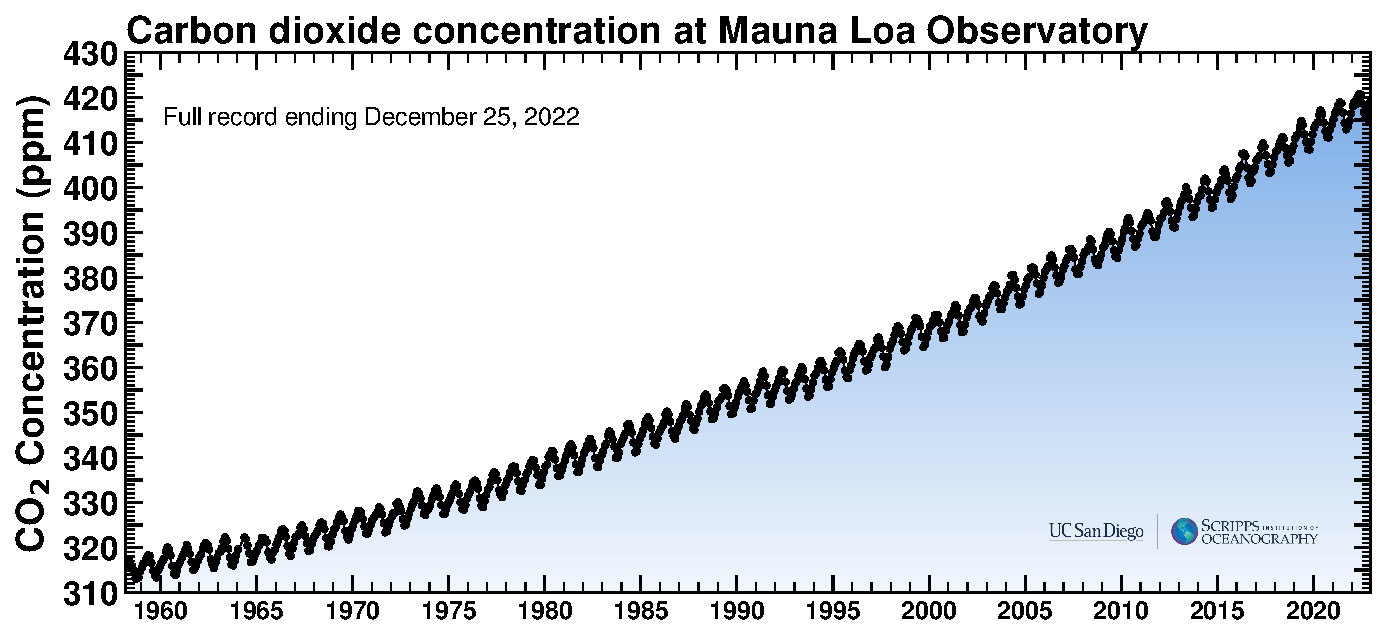
\includegraphics[width=1.0\textwidth,keepaspectratio,trim=0 0 0 0, clip]{figures/mlo_full_record.pdf}
%     \caption{ Mauna Loa observatory \ch{CO2} measurement \parencite{keeling-curve} }
%     \label{fig:scatter_plot_sand}
% \end{figure}


% \section{Example chemical reaction}
% Carbonic acid deprotonation:
% \begin{equation}
%     \ch{CO2 + H2O ->[] HCO3^- + H^+}.
% \end{equation}

% \section{Example of the equation with self-defined conditions environment }
% The relative permittivity $\epsilon_{r}$ is defined as: 
% \begin{equation}
%     \label{eqn:relative_permittivity}
%     {\displaystyle \varepsilon _{\mathrm {r} }={\frac {\varepsilon }{\varepsilon _{0}}}}
% \end{equation}
% \begin{conditions}
%     \epsilon & permittivity of the material \\
%     \epsilon_0 & vacuum permittivity.\\
% \end{conditions}

% \section{Example of different citations}
% Overall \textcite{arrhenius1896xxxi} calculated that cutting CO2 in half would suffice to produce an ice age. He further calculated that a doubling of atmospheric CO2 would give a total warming of 5–6 degrees Celsius.

% \noindent
% Overall, Arrhenius calculated that cutting CO2 in half would suffice to produce an ice age. He further calculated that a doubling of atmospheric CO2 would give a total warming of 5–6 degrees Celsius (\cite{arrhenius1896xxxi}).

% \noindent
% Overall, Arrhenius calculated that cutting CO2 in half would suffice to produce an ice age. He further calculated that a doubling of atmospheric CO2 would give a total warming of 5–6 degrees Celsius \parencite{arrhenius1896xxxi}.

% \section{Example list}
% \begin{itemize}
%     \item first
%     \item second
%     \item third
%     \item fourth
%     \item fifth
%     \item sixth
%     \item seventh
% \end{itemize}

% \section{Example table}

% \begin{table}[H]
% \centering
% \begin{tabular}{|l|l|}
% \hline
% \rowcolor{gray!50}
% Country (or dependency) & Population (2020) \\ \hline
% China                  & 1,439,323,776       \\ \hline
% India                  & 1,380,004,385        \\ \hline
% USA                    & 331,002,651           \\ \hline
% Indonesia              & 273,523,615            \\ \hline
% Pakistan               & 220,892,340             \\ \hline
% Brazil                 & 212,559,417              \\ \hline
% Nigeria                & 206,139,589               \\ \hline
% \end{tabular}
% \caption{example caption }
% \label{tbl:example_table}
% \end{table}

% \section{Example of siunitx package}
% The siunitx package is amazing for controlling all numbers and units of the document globally. You can set everything globally for the document and don't need to change every single number for formatting changes.\\
% At the beginning of the document, the settings are made.

% %% settings for the SI units from main.tex
% % \sisetup{locale = DE,
% % output-decimal-marker={.}, % because  in german is switched to {,}
% % separate-uncertainty=true,  
% % multi-part-units=single,
% % range-units = single ,  
% % list-units = single,  
% % per-mode=reciprocal,
% % group-minimum-digits = 4,
% % number-unit-product = \hspace{0.16667em plus 0.08334em}}



% \begin{itemize}
%     \item range of numbers + unit:  \SIrange{3}{10}{\cubic\kilo\meter \per \second}
%     \item number + unit : \SI{3}{\cubic\kilo\meter \per \second}
%     \item just unit   : \si{\cubic\kilo\meter \per \second}
%     \item number + uncertainty + unit \SI{3 \pm 0.1}{\cubic\kilo\meter \per \second}
% \end{itemize}

% \section{Example colors}
% Example of how to use colors in the text.
% \begin{enumerate}
% \color{blue}
%     \item Blue
%     \item More blue
%     \item {\color{red} And red!}
%     \item \begingroup\color{green} lol   \endgroup
%     \item {\color{yellow} And yellow!}
% \end{enumerate}


